\documentclass[xcolor=dvipsnames,10pt]{beamer}

\beamersetaveragebackground{blue!10}

\mode<presentation>
{
     \usetheme{Warsaw}
}

\usepackage{polski}
\RequirePackage[utf8]{inputenc}

\author{Joanna Kotuła, Aleksandra Murawska}
\institute[...]{Wydział Matematyki, Informatyki i Mechaniki\\
Uniwersytet Warszawski}

\subject{...}

\title[Intuicyjny język wyszukiwania TQL (Tablets Query Language)]{\bf  Intuicyjny język wyszukiwania TQL \\
Tablets Query Language}
%\subtitle{...}

\date{\today}



\begin{document}


\begin{frame}
     \titlepage
\end{frame}

%\begin{frame}
%     \frametitle{Spis treści}
%     \tableofcontents
%\end{frame}



\section{Domain Specific Languages}


\begin{frame}
     \frametitle{Domain Specific Languages (DSL)}
     
     DSL to języki przystosowane do używania w konkretnym celu.
     \begin{itemize}
          \item
          łatwość użycia
          \item
          specyficzne konstrukcje
          \item 
          ograniczone możliwości
          \item
          kompilacja do języka niższego poziomu (np. SQL)
     \end{itemize}


\end{frame}

\section{Tabliczki sumeryjskie}
%Coś o sumerach


\begin{frame}
     \frametitle{Tabliczki sumeryjskie}

\begin{columns}
\column{0.5\textwidth}
\begin{itemize}
\item gliniane tabliczki pokryte pismem klinowym
\item pochodzą z terenów Bliskiego Wschodu
\item najstarsze znane pismo (powstało ok. 3500r. p.n.e.)
%\item wiele zachowało się dzięki pożarom, ważniejsze wypalano specjalnie
%\item odciskane rylcem o trójkątnym przekroju
\item pismo początkowo rysunkowe, później coraz prostsze
\item głównie teksty gospodarcze i administracyjne% (dość regularne i rzeczowe)

\end{itemize}
\column{0.5\textwidth}
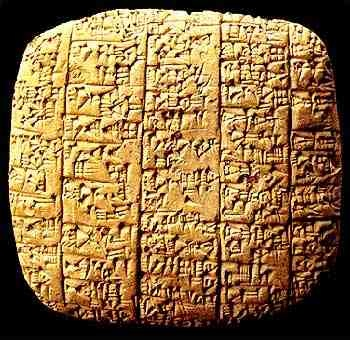
\includegraphics[width=55mm]{tablet.jpg}
\end{columns}
\end{frame}



\begin{frame}
\frametitle{Sumerologia}
    
\begin{columns}
 \column{0.5\textwidth}
Sumerologia to nauka badająca kulturę i historię starożytnych Sumerów, czerpiąca wiedzę m.in. z zachowanych tabliczek.
\begin{itemize}
\item zdigitalizowane i ręcznie skorygowane treści tabliczek są udostępnione przez system CDLI (obecnie prawie 225 000 tabliczek)
\item możliwość niewłaściwej interpretacji klinów
\item potrzebne intuicyjne narzędzie do wyszukiwania w bazie tabliczek na podstawie odczytów
\end{itemize} 

  \column{0.5\textwidth}
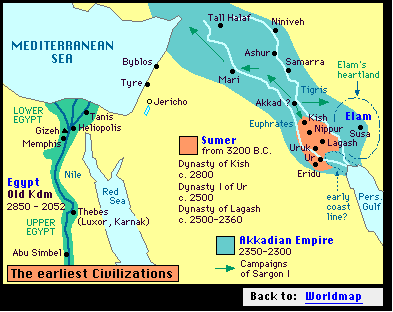
\includegraphics[width=55mm]{sum_map.png}
\end{columns}


\end{frame}


\section{Tablets Query Language}


\begin{frame}
     \frametitle{Tablets Query Language}
     \begin{itemize}
    \item Język pozwalający sumerologom łatwo tworzyć zapytania w bazie tabliczek.\\
   \item  Prosta składnia zapytań.\\
 \item    Zapytania zawierają informacje tylko o treści tabliczek i ich metadanych.\\
  \item   Możliwość stworzenia implementacji na dowolną bazę przechowującą tabliczki.\\ %ułatwiamy to dzięki podziałowi kodu na moduły

 \end{itemize}

\end{frame}
 
\begin{frame}

% dać składnię

     \frametitle{Przykładowe zapytania TQL}

\begin{block}{przykład 1}

provenience: Ur*\\
period: "Uruk III"\\
genre: Administrative\\
text: udu + (szid / sipa) $--$ adad-tilati\\

\end{block}
\end{frame}



\begin{frame}

     \frametitle{Przykładowe zapytania TQL}

\begin{block}{przykład 2}

provenience: Gar*\\
period: UrIII\\
genre: Administrative\\
text: udu/masz2\\
~\\
provenience: Ur\\
period: UrIII\\
text: sig4\\
\end{block}
\end{frame}



\begin{frame}
 \frametitle{Przykładowe zapytania TQL}

\begin{block}{przykład 3}

define\\
  provenience: Garshana\\
  period: UrIII\\
  text: "udu ban"/mash2\\
as "zwierzaki w Garshana"\\
~\\
search\\
  text: adad-tilati\\
in "zwierzaki w Garshana"\\

\end{block}

\end{frame}




\section{Struktura translatora}
% Struktura translatora, opisać co się dzieje, dlaczego jest niezależne 
% itp., przepływ zapytania przez program




\begin{frame}
     \frametitle{Podział na moduły}
     
\begin{center}
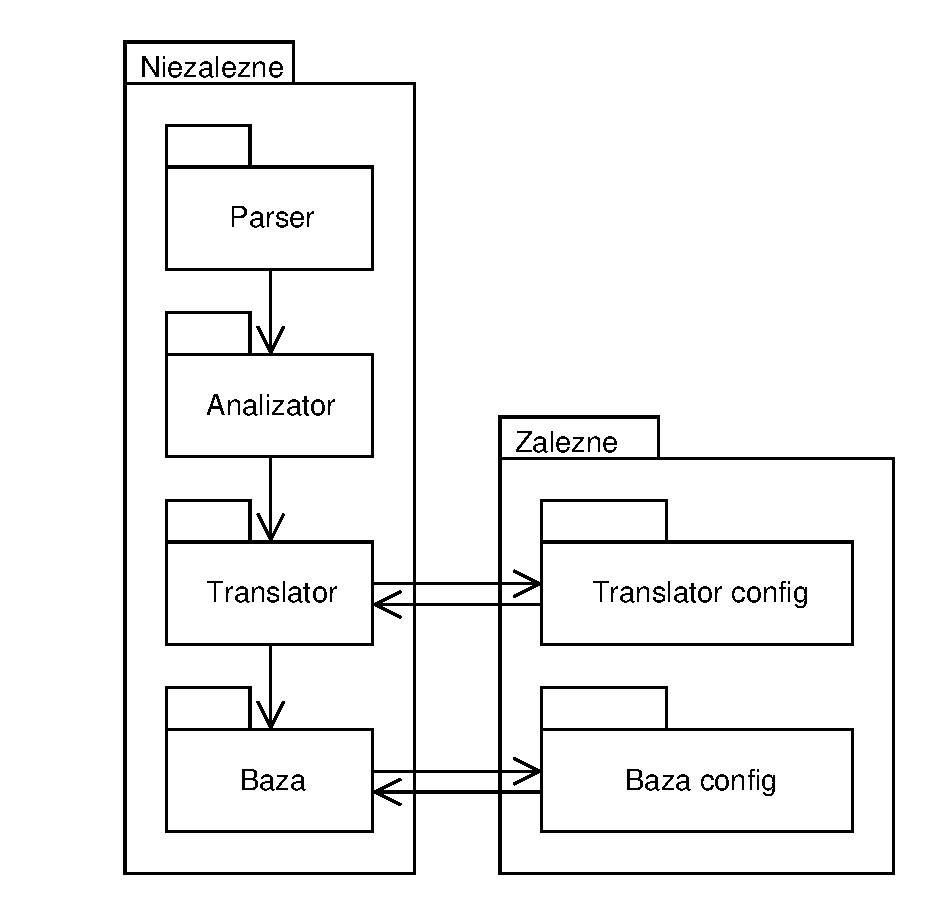
\includegraphics[height=70mm]{pakiety.pdf}
%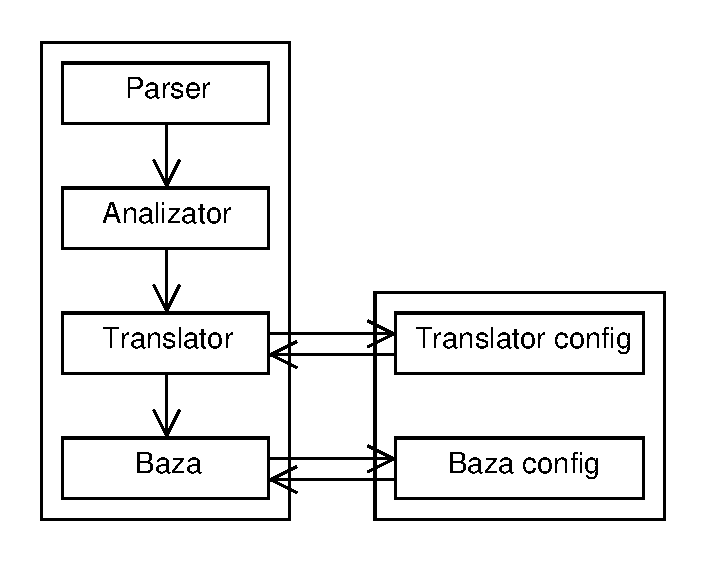
\includegraphics[height=70mm]{moduly.pdf}
\end{center}

\end{frame}

\begin{frame}
     \frametitle{Parser i analizator składniowy}
     
\begin{itemize}
\item moduły niezależne od bazy danych i języka wyszukiwania
\item wspólne dla wszystkich  implementacji TQL
\item wejście - zapytanie w języku TQL
\item wyjście - drzewo składni abstrakcyjnej

\end{itemize}


\end{frame}

\begin{frame}
     \frametitle{Translator}
     
\begin{itemize}
\item moduł zależny od języka docelowego
\item komunikuje się z modułem konfiguracyjnym, który zawiera funkcje tłumaczące poszczególne konstrukcje
\begin{itemize}
\item zapytanie
\item linia zapytania
\item i (+)
\item lub (/)
\item nie ($--$)
\item cokolwiek (*)
\end{itemize}
\item wejście - drzewo składni abstrakcyjnej
\item wyjście - zapytanie w odpowiednim języku

\end{itemize}


\end{frame}

\begin{frame}
     \frametitle{Baza}
     
\begin{itemize}
\item moduł zależny od wykorzystywanej bazy danych
\item komunikuje się z modułem konfiguracyjnym, który zawiera funkcję wykonującą zapytanie
\begin{itemize}
\item moduł konfiguracyjny zawiera oddzielny plik z danymi dostępu do bazy
\end{itemize}
\item przetwarza wynik zapytania do postaci XML
\item wejście - zapytanie w języku docelowym
\item wyjście - XML zawierający informacje o znalezionych tabliczkach i ich treść

\end{itemize}

\end{frame}

\begin{frame}
     \frametitle{Aplikacja wykorzystująca translator}
   
\begin{itemize}
\item umożliwa użytkownikowi wprowadzenie zapytania jako tekstu lub za pomocą graficznego interfejsu
\item odpowiednio wyświetla zwracanego XML-a, pokazując wyszukiwane sekwencje
\end{itemize}

\end{frame}


\section{Co zrobiłyśmy, co planujemy}
%  Problemy (?) planowane optymalizacje (coś ciekawego na pewno musi 
% być), featury (planowane)


\begin{frame}
     \frametitle{Do tej pory}
     
\begin{itemize}
\item przykładowa baza relacyjna (Postgres)
\item gotowy parser i analizator składniowy
\item moduł translatora i moduł konfiguracyjny dla bazy relacyjnej
\item moduł bazy: połączenie z bazą, wykonywanie zapytań i zwracanie XML-a -- jeszcze bez zaznaczonych sekwencji wyszukiwania
\end{itemize}


\end{frame}

\begin{frame}
     \frametitle{Plany}
     
\begin{itemize}
\item zaznaczanie w XML-u z tabliczkami wyszukiwanych sekwencji
\item interfejs graficzny -- do wprowadzania zapytań i wyświetlania wyników
\item moduły konfiguracyjne do innej bazy danych
\item optymalizacje zapytań (obowiązkowo dla negacji)
\item tłumaczenie odczyty $\leftrightarrow$  kliny i wyszukiwanie po klinach
\end{itemize}
\end{frame}

%\section{Pokaz działania}

%\begin{frame}
%     \frametitle{Pokaz działania}
%\end{frame}


\end{document}




